% Search for all the places that say "PUT SOMETHING HERE".

\documentclass[11pt]{article}
\usepackage{amsmath,textcomp,amssymb,geometry,graphicx,enumerate}
\usepackage{ctex}

\def\Name{了然}  % Your name
\def\SID{2016302580055}  % Your student ID number
\def\Homework{1} % Number of Homework
\def\Session{Spring 2019}


\title{\Large Networks and Distributed Computing --- Spring 2019 --- Homework \Homework\ }
\author{\Name, Student ID: \SID}
\markboth{Networks and Distributed Computing--\Session\  Homework \Homework\ \Name}{Networks and Distributed Computing--\Session\ Homework \Homework\ \Name}
\pagestyle{myheadings}
\date{\today}

\newenvironment{qparts}{\begin{enumerate}[{(}a{)}]}{\end{enumerate}}
\def\endproofmark{$\Box$}
\newenvironment{proof}{\par{\bf Proof}:}{\endproofmark\smallskip}

\textheight=9in
\textwidth=6.5in
\topmargin=-.75in
\oddsidemargin=0.25in
\evensidemargin=0.25in


\begin{document}
\maketitle

\section{Ping}

\begin{figure}[h]
\centering
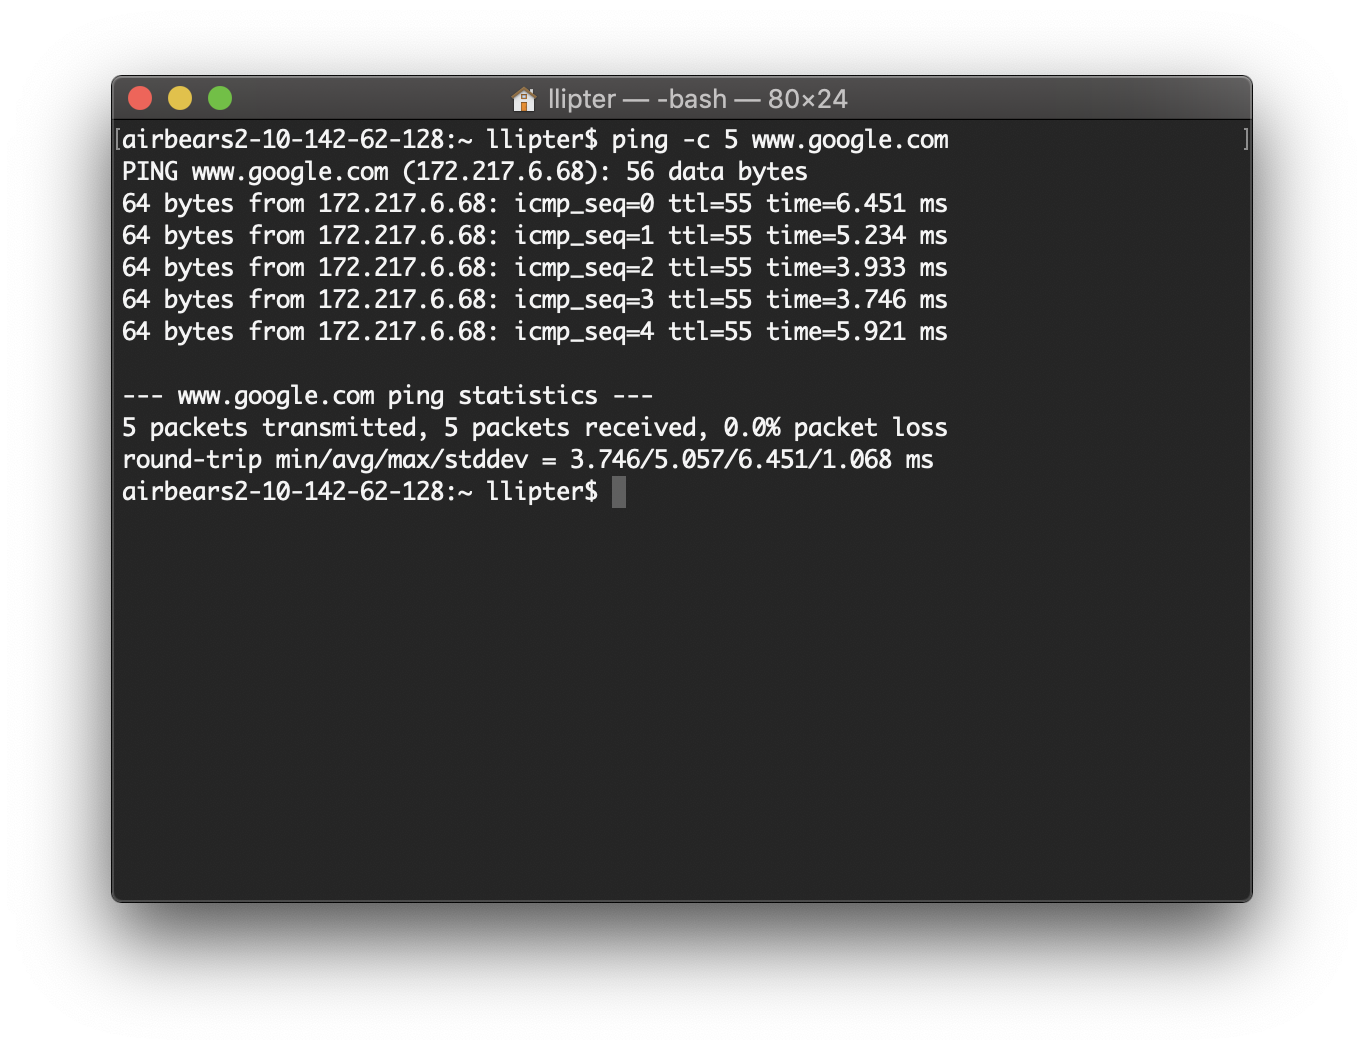
\includegraphics[width=1\textwidth]{ping.png}
\caption{\label{fig:ping}Ping Google}
\end{figure}

\newpage
\section{Traceroute}

\begin{figure}[h]
\centering
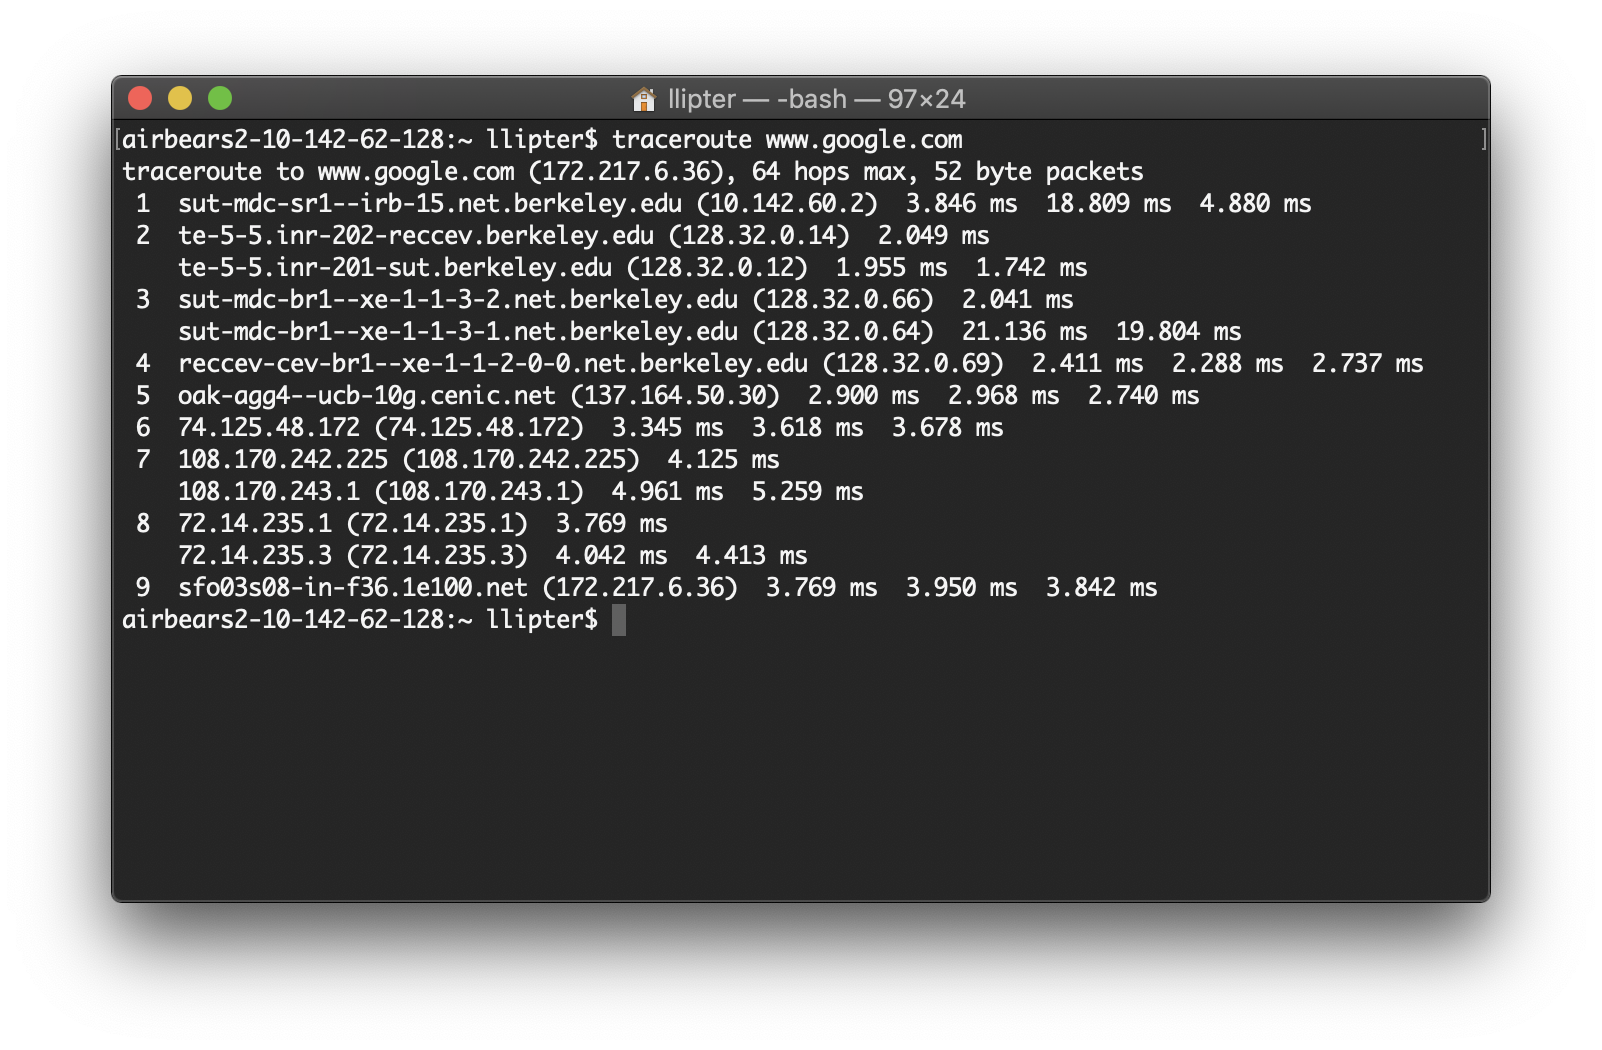
\includegraphics[width=1\textwidth]{traceroute.png}
\caption{\label{fig:traceroute}Tracerout Google}
\end{figure}

\newpage
\section{Problem 6}

This elementary problem begins to explore propagation delay and transmis- sion delay, two central concepts in data networking. Consider two hosts, A and B, connected by a single link of rate R bps. Suppose that the two hosts are separated by m meters, and suppose the propagation speed along the link is s meters/sec. Host A is to send a packet of size L bits to Host B.

\begin{qparts}

	\item \textbf{Express the propagation delay, $d_{prop}$, in terms of $m$ and $s$.}
	
	$d_{prop} = \frac{m}{s}$
	
	\item \textbf{Determine the transmission time of the packet, $d_{trans}$, in terms of $L$ and $R$.}

	$d_{trans} = \frac{L}{R}$
	
	\item \textbf{Ignoring processing and queuing delays, obtain an expression for the end- to-end delay.}
	
	$d_{end-to-end} = d_{prop} + d_{trans} = \frac{m}{s} + \frac{L}{R}$
	
	\item \textbf{Suppose Host A begins to transmit the packet at time $t = 0$. At time $t = d_{trans}$, where is the last bit of the packet?}
	
	It just leaved A.
	
	\item \textbf{Suppose $d_{prop}$, is greater than $d_{trans}$. At time $t = d_{prop}$, where is the first bit of the packet?}

	It's still in the link and hasn't reach B.
	
	\item \textbf{Suppose $d_{prop}$ is less than $d_{trans}$. At time $t = d_{trans}$, where is the first bit of the packet?}
	
	It has reached B.
	
	\item \textbf{Suppose $s = 2.5 \times 10^8 , L = 120$ bits, and $R = 56$ kbps. Find the distance $m$ so that $d_{prop}$ equals $d_{trans}$.}
	
	$m =  \frac{L}{R} s = \frac{120}{56 \times 10^3}2.5 \times 10^8 \approx 5.36 \times 10^5$m

	

\end{qparts}



\newpage
\section{Problem 8}

Suppose users share a 3 Mbps link. Also suppose each user requires 150 kbps when transmitting, but each user transmits only 10 percent of the time. (See the discussion of packet switching versus circuit switching in Section 1.3.)

\begin{qparts}
	\item \textbf{When circuit switching is used, how many users can be supported?}
	
	Number of users supported = $\frac{3 \operatorname{Mbps}}{150 \operatorname{kbps}} = 20$

	\item  \textbf{For the remainder of this problem, suppose packet switching is used. Find the probability that a given user is transmitting.}
	
	$p = 0.1$
	
	\item  \textbf{Find the probability that at any given time, exactly \textit{n} users are transmitting simultaneously.(Hint: Use the binomial distribution.)}
	
	$P = \tbinom{120}{n}p^{n}(1-p)^{120-n}$
	
	\item  \textbf{Find the probability that there are 21 or more users transmitting simultaneously.}
	
	$P = 1 - \sum_{n=0}^{20} \tbinom{120}{n}p^{n}(1-p)^{120-n}$

\end{qparts}

\newpage
\section{Problem 9}

Consider the discussion in Section 1.3 of packet switching versus circuit switch- ing in which an example is provided with a 1 Mbps link. Users are generating data at a rate of 100 kbps when busy, but are busy generating data only with probability p = 0.1. Suppose that the 1 Mbps link is replaced by a 1 Gbps link.

\begin{qparts}
	\item \textbf{What is \textit{N}, the maximum number of users that can be supported simulta- neously under circuit switching?}
	
	$N = \frac{1 \operatorname{Gbps}}{100 \operatorname{kbps}} \frac{1}{p} = 100000$
	
	\item \textbf{Now consider packet switching and a user population of \textit{M} users. Give a formula (in terms of \textit{p, M, N}) for the probability that more than \textit{N} users are sending data.}
	
	$P = 1 - \sum_{n=0}^{N} \tbinom{M}{n}p^{n}(1-p)^{M-n}$

\end{qparts}


\end{document}